\subsection{Penjili \& \newspeak}

\begin{frame}{Le projet Penjili}
\centering
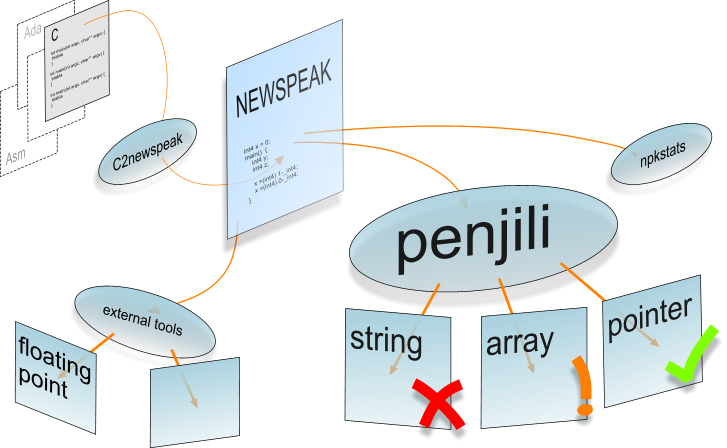
\includegraphics[scale=.5]{img/penjili.png}
\end{frame}

\begin{frame}{Le langage intermédiaire \newspeak}

Un langage adapté à l'analyse statique:

\begin{itemize}
\item simple: il contient peu de constructions
\item explicite: les effets de bords sont explicites
\item expressif: tout programme C peut être converti en \newspeak
\end{itemize}

\end{frame}

\begin{frame}[fragile]{Exemple}

\begin{SaveVerbatim}{compilnpk}
int32 x;
x =(int32) 0;
do {
    while (1) {
        choose {
            -->
                guard((10 > x_int32));
            -->
                guard(! (10 > x_int32));
                goto lbl1;
        }
        x =(int32) coerce[-2**31,2**31-1]
                        (x_int32 + 1);
    }
} with lbl1: {
}
\end{SaveVerbatim}

{\footnotesize
\begin{minipage}{0.3\linewidth}
\insertcode{npk-while.c}
\end{minipage}
\vrule\hspace{2pt}
\begin{minipage}{0.6\linewidth}
\BUseVerbatim{compilnpk}
\end{minipage}
}

\end{frame}

\begin{frame}{Compilation \& analyse}

\begin{tikzpicture}\shorthandoff{!}
\tikzstyle{file}=[draw, shape=rectangle, node distance=2.2cm, minimum
height=1cm, shade, top color=white,
    bottom color=blue!50!black!20, draw=blue!40!black!60, very thick];

\node [file] (c1) {\textcolor{black}{.c}};
\node [file, below of=c1] (c2) {\textcolor{black}{.c}};
\node [node distance=2.2cm, below of=c2] (c3) {};

\node [file, minimum height=0, node distance=5mm, above of=c3,draw] (c3b) {.adb};
\node [file, minimum height=0, node distance=5mm, below of=c3,draw] (c3s) {.ads};

\path (c3b.north west) ++(-3mm,3mm) [draw,dotted] rectangle ($(c3s.south east)+(3mm,-3mm)$);

\node [below of=c3, node distance=2.2cm] (c4){};

\node [file, right of=c1] (cc1) {\textcolor{black}{.c}};
\node [file, right of=c2] (cc2) {\textcolor{black}{.c}};
\node [node distance=2.2cm, right of=c3] (cc3) {};

\node [below of=cc3, node distance=2.2cm](cc4){};

\draw[->] (c1) -- node[above] {{\tiny \ttfamily cpp}} (cc1);
\draw[->] (c2) -- (cc2);

\node [file, right of=cc1] (no1) {\textcolor{black}{.no}};
\node [file, right of=cc2] (no2) {\textcolor{black}{.no}};
\node [file, right of=cc3] (no3) {\textcolor{black}{.no}};

\node [below of=no3, node distance=2.2cm](no4){};

\draw[->] (cc1) -- node[above] {{\tiny \ttfamily c2newspeak -c}} (no1);
\draw[->] (cc2) --  (no2);

\draw[->] ($ (c3b.north east)!0.5!(c3s.south east) + (3mm,0) $) -- node[above] {\tiny \ttfamily ada2newspeak -c} (no3);


\node [file, right of=no2] (npk) {\textcolor{black}{.npk}};

\node [right of=no3, node distance=2.2cm](npk2){};
\node [right of=no4, node distance=2.2cm](npk3){};

\node[draw, ellipse, right of=no2, minimum height=3cm]{};

\draw[->] (no1) -- node {} (npk);
\draw[->] (no2) -- node[above] {{\tiny \ttfamily c2newspeak}} (npk);
\draw[->] (no3) -- node {} (npk);


\node [file, right of=npk, node distance=3cm, yshift=1cm](warn)
    {\textcolor{black}{\parbox{2cm}{\centering Programme \linebreak typé}}};
\node [right of=npk, node distance=3cm, yshift=-1cm](warnn)
    {\textcolor{black}{Erreurs}};

\node [right of=npk3, node distance=3cm](analyser2){};

\node [right of=npk, node distance=3cm] {\small ou};

\draw[->] (npk) -- node[above, yshift=2mm] {{\tiny \ttfamily ptrtype}} (warn);

\draw[->] (npk) -- (warnn);

\draw[->] (c4)   -- node[above, text depth=3pt] {\footnotesize Pr\'etraitement} (cc4);
\draw[->] (cc4)  -- node[above, text depth=3pt] {\footnotesize Compilation} (no4);
\draw[->] (no4)  -- node[above, text depth=3pt] {\footnotesize \'Edition de liens} (npk3);
\draw[->] (npk3) -- node[above, text depth=3pt] {\footnotesize Analyse} (analyser2);
\end{tikzpicture}


\end{frame}
